\problemname{Minerāļu atradnes}

\illustration{.3}{img/turnbull.jpg}{Erodējošs iezis ar jauniem minerāļiem. Foto: Michael D.\ Turnbull, license: CC BY-SA.}

\noindent
Jūs pārvaldāt signālu apstrādi ārpuszemes kalnrūpniecības uzņēmumam, un jūsu kuģis pašlaik tuvojas asteroīdam. Sākotnējās izlūkošanās dati rāda, ka asteroīdā atrodas $k$ minerālvielu atradnes, bet to precīzas atrašanās vietas nav zināmas.

\medskip

Asteroīda virsmu var uzskatīt par koordinātu režģi ar veselām koordinātēm.
Katra minerāļu atradne atrodas nezināmās veselās koordinātēs, kur $i$-tajai vietai ir koordinātas $(x_i, y_i)$ un
$-b \le x_i \le b$ un $-b\le y_i \le b$ %constraint:depositcoords
kādam veselam skaitlim $b$, kas atbilst jūsu sākotnējās  izlūkošanās izmēram.

Lai noteiktu minerālu atradņu precīzas atrašanās vietas, jūs varat sūtīt zondes uz asteroīda virsmas.
Zondes tiek sūtītas viļņos no vairākām zondēm vienlaikus.

Pieņemsim, ka jūs nosūtījāt vilni ar $d$ zondēm uz virsmas koordinātēm $(s_j, t_j)$ katram $1\leq j\leq d$.
Kad zonde sasniedz savas koordinātes, tā nosaka Manhetenas attālumus līdz katrai no $k$ minerāļu atradnēm un nosūta attālumus atpakaļ uz kuģi.
Visi dati no zondēm tiek saņemti uz kuģa vienlaikus, un nav iespējams noteikt, kuras zondes nosūtīja kurus attālumus.
Tādējādi viens vilnis atgriež $k\cdot d$ veselus attālumus
\[|x_i-s_j| + |y_i - t_j| \qquad\text{visiem } i \in \{1,\ldots,k\} \text{ un } j \in\{ 1,\ldots,d\}\,.\]

Jums nepieciešams minimizēt zonžu viļņu skaitu, kas ir nosūtīti uz virsmas pārbaudi.


\section*{Komunikācija}

Šis ir interaktīvs uzdevums.
Komunikācija sākas, kad nolasāt vienu rindu ar trīs veseliem skaitļiem $b$, $k$ un $w$:
režģa robeža~$b$,
minerāļu atradņu skaits~$k$
un maksimālais viļņu skaits~$w$, ko jūs drīkstat nosūtīt.

Pēc tam jūs uzdodat ne vairāk kā $w$ vaicājumus, kur katrs atbilst vienam vilnim.
Vaicājums sastāv no simbola \texttt{?}, kuram seko $2d$ veseli ar atstarpi atdalīti veseli skaitļi, piemēram ``\texttt{?} $s_1$ $t_1$ $\cdots$ $s_d$ $t_d$'', kur zonžu skaitam~$d$ šajā vilnī jāapmierina
$1\leq d\leq 2000$. % constraint:wavesize
Vērtības $(s_i, t_i)$ tiek interpretētas kā $i$-tās zondes koordinātas un tām jāapmierina
$-10^8 \leq s_i \leq 10^8$ un $-10^8 \leq t_i \leq 10^8$. % constraint:probecoordinates
Atbilde uz vaicājumu ir viena rinda ar $k \cdot d$ veseliem skaitļiem augošā secībā: visi Manhetenas attālumi starp minerāļu atradnēm un zonžu koordinātām.
Kopējais zonžu skaits visos viļņos kopā nedrīkst pārsniegt
$2\cdot 10^4$. % constraint:totalprobes

Komunikācija beidzas ar to, ka jūs izdrukājat vienu rindu, kas sastāv no \texttt{!}, pēc kuras seko $k$ punkti $x_1$, $y_1$, $x_2$, $y_2$, $\ldots$, $x_k$, $y_k$, kas ir atdalīti ar atstarpi.
Šai jābūt jūsu izvada pēdējai rindai.

Jūsu risinājums tiks uzskatīts par pareizu, ja jūs izvadīsiet visas minerāļu atradņu atrašanās vietu koordinātas.
Jūs varat tās izdrukāt jebkurā secībā.

\section*{Ierobežojumi un vērtēšana}

Vienmēr izpildās ierobežojumi
$1\leq b \leq 10^8$, % constraint:b
$1 \leq k \leq 20$, % constraint:k
and
$2 \le w \le 10^4$. % constraint:w

Jūsu risinājums tiks pārbaudīts uz vairākām testu grupām. Katra grupa ir vērta noteiktu punktu skaitu.
Katra testu grupa satur vairākus testus.
Lai saņemtu punktus par testu grupu, ir jāatrisina visi testi testu grupā.
Jūsu gala rezultāts būs lielākais punktu skaits, kas iegūts ar vienu risinājuma iesniegumu.

\medskip
\begin{tabular}{lll}
Grupa & Punkti & Ierobežojumi \\\hline
  $1$ & $9$ & $k = 1, w = 10^4$, $b \le 10^7$\\
  $2$ & $19$ & $w \ge 500$, $b \le 10^7$\\
  $3$ & $11$ & $w \ge 210$, $b \le 10^7$\\
  $4$ & $7$ & $w \ge 130$, $b \le 10^7$\\
  $5$ & $20$ & $w \ge 3$, $b \le 10^4$\\
  $6$ & $15$ & $w \ge 3$, $b \le 10^7$\\
  $7$ & $19$ & \emph{Bez papildu ierobežojumiem}
\end{tabular}

\section*{Piemērs}

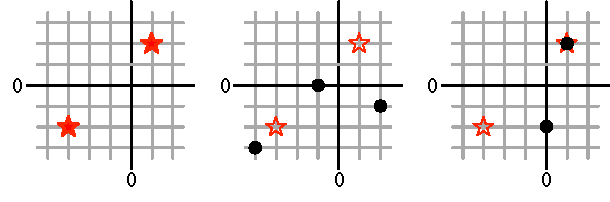
\includegraphics[width=.6\textwidth]{img/sample1.pdf}

Šajā piemērā ir $k=2$ minerāļu atradnes, kas atrodas pozīcijās $(1,2)$ un $(-3,-2)$, attēlotas ar sarkanām zvaigznītēm.
Pirmajā vilnī jūs varētu sūtīt $d=3$ zondes uz $(-4,-3)$, $(-1, 0)$ un $(2,-1)$, kas ir attēlotas kā melni punkti.
Šis vilnis atgrieztu $6$ attālumus \[
  2, 4, 4, 4, 6, 10\,.
\]
Nākamajā vilnī jūs varētu sūtīt $d=2$ zondes uz $(1,2)$ un $(0,-2)$.
Šī vilnis atgrieztu $4$ attālumus \[
  0, 3, 5, 8\,.
\]
